\documentclass[addpoints]{exam}
%%%%%%%%%%%%%%%%%% PACKAGES %%%%%%%%%%%%%%%%%%%%%%%%
\usepackage{amsmath}
\usepackage{amsfonts}
\usepackage{tcolorbox}
\tcbuselibrary{skins}
\usepackage{tikz,tkz-euclide,tikz-3dplot}
\usepackage{rotating}
%%%%%%%%%%%%%%%%%%%%%% MARGINS%% %%%%%%%%%%%%%%%%%%%
\extrawidth{.5in}
\extraheadheight{-.25in}
\extrafootheight{-.25in}
%%%%%%%%%%%%%%%%%% ANSWERS AND POINTS %%%%%%%%%%%%%%
%\printanswers
\pointsinrightmargin
\bracketedpoints
%%%%%%%%%%%%%%%%%% HEADER AND FOOTER %%%%%%%%%%%%%%%
\pagestyle{headandfoot}
\firstpageheadrule
\runningheadrule
\firstpageheader{\S4.A.2 Sequences and Series}{}{AP Precalc\\Mr. Carey}
\runningheader{\S4.A.2 Sequences and Series}{}{Mr. Carey}
\firstpagefooter{}{}{}
\runningfooter{ }{\thepage}{ }
%%%%%%%%%%%%%%%%%%%%%% NOTES %%%%%%%%%%%%%%%%%%%%%%%

%%%%%%%%%%%%%%%%%% DOCUMENT CONTENTS %%%%%%%%%%%%%%%
\begin{document}
\section*{Practice}
\begin{questions}
    \question The values of a sequence $g_n$ are given in the graph below.
    \begin{center}
    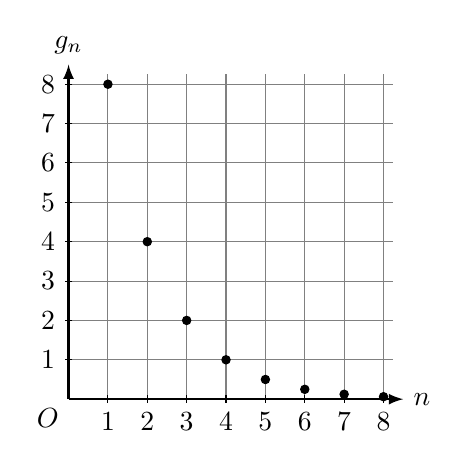
\begin{tikzpicture}[scale=.5]
        \draw[color=gray] (0,0) grid (8.25,8.25);
        \draw[thick,-latex] (0,0) -- (8.5,0) node[anchor=west]{$n$};
        \draw[thick,-latex] (0,0) -- (0,8.5) node[anchor=south]{$g_n$};
        \node[anchor=north east] at (0,0){$O$};
        \foreach \x in {1,2,...,8}
            \draw (\x,.1) -- (\x,-.1) node[anchor=north]{$\x$};
        \foreach \y in {1,2,...,8}
            \draw (.1,\y) -- (-.1,\y) node[anchor=east]{$\y$};
        \draw[fill=black] (1,8) circle (3pt);
        \draw[fill=black] (2,4) circle (3pt);
        \draw[fill=black] (3,2) circle (3pt);
        \draw[fill=black] (4,1) circle (3pt);
        \draw[fill=black] (5,.5) circle (3pt);
        \draw[fill=black] (6,.25) circle (3pt);
        \draw[fill=black] (7,.125) circle (3pt);
        \draw[fill=black] (8,.0625) circle (3pt);
        
    \end{tikzpicture}
    \end{center}
    Answer each of the following.
    \begin{parts}
        \part Find a formula for the $n$th term of the sequence.
        
        \vspace{\stretch{.5}}

        \part Does the sum $\displaystyle\sum_{n=1}^\infty g_n$ converge? If so, what is the sum?

        \vspace{\stretch{.5}}
    \end{parts}

    \question The terms of an increasing arithmetic sequence $a_n$ are positive. The terms of the increasing geometric sequence $b_n$ are positive. The values of the first term of both sequences are the same, and the values of the fourth terms are the same. Which of the following statements describes the values of the second terms of the sequences?
    \begin{choices}
        \choice The second term of the arithmetic sequence must be less than the second term of the geometric sequence.
        \choice The second term of the arithmetic sequence must be greater than the second term of the geometric sequence.
        \choice The second term of the arithmetic sequence must be equal to the second term of the geometric sequence.
        \choice The relationship between the values of the second terms cannot be determined from the given information.
    \end{choices}

    \vspace{\stretch{.5}}

    \question Consecuative terms of a sequence have the values $6,\,2,\,-2,\,-6,\ldots$. What is the sum of the first 100 terms of the sequence?

    \vspace{\stretch{1}}

    \newpage

    \question Determine if the following sequences are arithmetic, geometric, or neither. For all, find a formula (explicit or recursive) for the sequence.
    \begin{parts}
        \begin{minipage}{.3\linewidth}
            \part $\displaystyle 1,\,3,\,5,\,7,\,9,\ldots$   
        \end{minipage}
        \hfill
        \begin{minipage}{.3\linewidth}
            \part $\displaystyle 2,\,4,\,8,\,16,\,32,\ldots$
        \end{minipage}
        \hfill
        \begin{minipage}{.3\linewidth}
            \part $\displaystyle 1^2,\,2^2,\,3^2,\ldots$
        \end{minipage}

        \vspace{\stretch{1}}

        \begin{minipage}{.3\linewidth}
            \part $\displaystyle 2,\frac{4}{\sqrt{3}},\frac{8}{3},\frac{16}{3\sqrt{3}},\ldots$
        \end{minipage}
        \hfill
        \begin{minipage}{.3\linewidth}
            \part $\displaystyle \frac{1}{2},\,\frac{1}{3},\,\frac{1}{4},\,\frac{1}{5},\,\ldots$
        \end{minipage}
        \hfill
        \begin{minipage}{.3\linewidth}
            \part $\displaystyle \frac{5}{4},\,\frac{3}{2},\,\frac{7}{4},\,2,\,\frac{9}{4},\,\ldots$
        \end{minipage}

        \vspace{\stretch{1}}

        \begin{minipage}[t]{.3\linewidth}
            \part $\displaystyle \frac{1}{2},\,\frac{3}{4},\,\frac{5}{6},\,\frac{7}{8},\,\ldots$
        \end{minipage}
        \hfill
        \begin{minipage}[t]{.3\linewidth}
            \part $\displaystyle 1,\,0.9,\,0.99,\,0.999,\,\ldots$
        \end{minipage}
        \hfill
        \begin{minipage}[t]{.3\linewidth}
            \part Write a seqence with positve and negative terms that has a sum less than zero.
        \end{minipage}

        \vspace{\stretch{1}}

        

        
    \end{parts}
\end{questions}





\end{document}